
\chapter{Building and running TWOPEG}
\label{sect:inp_param}
%Input file with parameters description.
%Output to BOS for backward compatibility with CLAS.
%Compilation with and without BOS libraries (needs to be done).
%Table with LUND output description.


TWOPEG has two compiling options. 
\begin{itemize}
 
\item "make nobos" compiles without BOS libraries, no output in BOS format is possible in this case.
 
\item "make bos" compiles with BOS libraries. BOS output can be created according to the flag in the input file. Special libraries needed for this option are not available among the standard CLAS libraries on ifarm machines anymore.  So, they were compiled manually and located  at this path "$\sim$gleb/lib/LinuxRHFC8", which is specified in the MakeFile. Since these libraries are not supported, sooner or later they will become irrelevant.
\end{itemize}

\begin{figure}[!ht]
\begin{center}
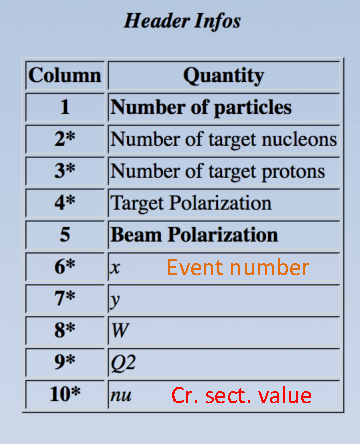
\includegraphics[width=0.25\textwidth]{pictures/inpparam/lund_out.pdf}
\end{center}
\vspace{-0.6cm}
\caption{\small The event header in LUND format output. Quantities marked with stars are not used by GEMC, but are still kept in the output stream (user defined meanings could be assigned to them).}
\label{fig:lund_out}
\end{figure}

The compilation and running was tested on ifarm machines.

After the compilation is complete, to run TWOPEG one should type "twopeg\_bos~$<$~inp1" or "twopeg\_nobos $<$ inp1" depending on the compiling options.

The input file "inp1" is located in the EG root directory. It contains input parameters with some comments. In more details these parameters are explained in Tabl.~\ref{tab:input_par}. 



\begin{table}[h]\scriptsize
\begin{center}
  \renewcommand{\arraystretch}{1.2}
\begin{tabular}{|c|l|}

\hline
Input parameter & Description\\
\hline 
$N_{evt}$ & Number of events to be generated \\
\hline
$E_{beam}$ & Beam energy (GeV) \\
\hline
$W_{min}$ & W minimum (GeV) \\
\hline
$W_{max}$& W maximum (GeV) \\
\hline
$Q^{2}_{min}$ & $Q^{2}$ minimum (GeV$^2$) \\
\hline
$Q^{2}_{max}$     & $Q^2$ maximum (GeV$^2$) \\
\hline 
$\theta_{min}$ & Minimal $\theta$ of the scattered electron (deg)\\
\hline 
 $\theta_{max}$  & Maximal $\theta$ of the scattered electron (deg)\\
\hline 
$E_{min}$ & Minimal energy of the scattered electron (GeV)\\
\hline 
$R_{targ}$  & Target radius in cm \\
\hline
$L_{targ}$ & Target length in cm \\
\hline
$Z^{off}_{targ}$ & Target offset in $z$ in cm\\
\hline
$\rho_{targ}$ & Target density (g/cm$^3$)\\
\hline
$l^{rad}_{targ}$  & Target radiation length (cm)\\
\hline
$Z_{targ}$ & Target $Z$\\
\hline
$A_{targ}$ & Target $A$\\
\hline
$Th_{wi}$,  $Th_{wf}$   & Thickness of the target windows initial, final (um)\\
\hline
$\rho_{wi}$, $\rho_{wf}$   & Density of target windows initial,final (g/cm$^3$)\\
\hline
$l^{rad}_{wi}$, $l^{rad}_{wf}$  & Radiation length of target windows initial,final (cm)\\
\hline
 &  Output BOS file: 0 - no,\\
$F_{bos}$   &  1 - MCTK,MCVX banks,\\
 &  2 - PART bank\\
\hline
out.bos     & BOS output file name\\
\hline
$F_{lund}$  & Otput LUND file 0 - no, 1 - yes\\
\hline
out.lund    & LUND output file name\\
\hline
 & Radiative mode: 0 - no rad effects,\\
$F_{rad}$   & 1 - rad eff with no straggling, \\ 
 & 2 - rad eff with straggling\\
\hline
$F_{fermi}$  & Fermi smearing: 0 - no, 1 - yes\\
\hline
 &Multiplication by virtual photon flux:\\
$F_{flux}$   &0 - no (under influence of virtual photons),\\
&1 - yes (under influence of electrons)\\
\hline
\end{tabular}
\caption{\small List of the input parameters and their description. \label{tab:input_par}}
\end{center}
\end{table}



The generator produces output in the LUND format. The header of the event was slightly changed in comparison with the conventional one that is used in GEMC. In the field six the event number is placed instead of "x" and in the field ten the cross section value is placed instead of "nu"  (see Fig.~\ref{fig:lund_out}). An example of LUND output for two double pion events generated with TWOPEG is given in Fig.~\ref{fig:evnt_exmpl}.

\begin{figure}[!ht]
\begin{center}
%\frame{
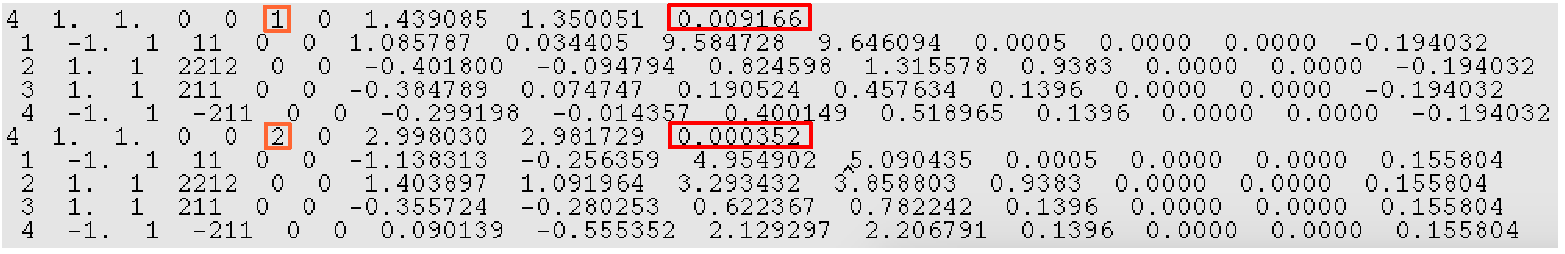
\includegraphics[width=1.\textwidth]{pictures/inpparam/events_exmpl.pdf}
%}
\end{center}
\caption{\small Example of two generated double pion events. The event numbers are in the orange boxes, while the weights are in the red boxes.}
\label{fig:evnt_exmpl}
\end{figure}

For the backward compatibility with CLAS software TWOPEG can also produce  output in BOS format. In this case there are two options in the input file: the option with $F_{bos}=1$ serves to generate "MCTK" and "MCVX" banks, while the other option with $F_{bos}=2$ is needed to generate the "PART" bank.




TWOPEG needs ".dat" files with tabulated structure functions and fit parameters. They are located in the "data" subfolder inside the EG root directory. If one needs to move it, one should define the environment variable "data\_dir\_2pi" that points to the new "data" folder location (for example in csh one should use "setenv data\_dir\_2pi new\_path/").


There are also two ".root" output files: the first one contains the root tree with the weights for each event and the second one contains some histograms, which one may find useful for the purpose of a quick check of the kinematical coverage, distributions of EG yield, etc.
